\documentclass[11pt]{article}
\usepackage[margin=1in]{geometry}
\usepackage{graphicx}
\usepackage{booktabs}
\usepackage{amsmath}
\usepackage{amssymb}
\usepackage{xcolor}
\usepackage[hidelinks]{hyperref}
\usepackage{caption}
\captionsetup{font=small}

\newcommand{\reconear}{\texttt{reco\_near}}
\newcommand{\recofar}{\texttt{reco\_far}}

\title{\vspace{-2.5em}Detector~3 position misses: reference-tracker error,
edges, and the passivated area\\
\large (June cosmic bench, \textbf{M3 v2} basis --- \texttt{g\_det3\_wknd}, cross-checked on \texttt{sat\_det3})}
\author{MX17 cosmic-bench QA}
\date{\today}

\begin{document}
\maketitle
\vspace{-1.5em}

\noindent\textbf{Supersedes} the pre-v2 \texttt{main.pdf} in this directory (which used the
$\chi^2<20$ ray recipe and reported a $13.7\,\%$ edge-concentrated \recofar\ tail). On the
current v2 recipe ($\chi^2<5$, NClus$\ge3$) that tail is halved, is \emph{not} edge-enhanced,
and is roughly half attributable to the reference tracker. This note answers three questions
the owner asked: (1) are the $>\!2$~mm misses the \emph{reference tracker's} fault?
(2) do they correlate with detector \emph{edges}? (3) is the $\sim2$~cm \emph{passivated} $Y$
strip properly handled in the efficiency.

\section{Setup}
For every clean M3 reference muon crossing the det3 active area we classify the detector's
response exactly as \texttt{09\_efficiency\_breakdown.py} does (same alignment, active box, and
$>\!50$-strip spark veto removed \emph{before} the reco/hit split): \reconear\ ($|r|\le5$~mm),
\recofar\ ($|r|>5$~mm), \texttt{spark}, \texttt{hit\_no\_reco}, \texttt{no\_hit}. The headline
run reproduces the June overview PDF exactly: $88.8\%$ \reconear, $6.5\%$ \recofar, $4.4\%$
spark. Of \emph{reconstructed} hits, $93.2\%$ land within $5$~mm, core $\sigma(|r|<15)=0.63$~mm,
median $|r|=1.01$~mm. Here we additionally record, per crossing, the \textbf{M3 reference-track
quality} (Chi2X, Chi2Y, NClusX/Y, incidence angle) and map every ray into the
\textbf{detector-local strip frame} ($0$--$399$~mm) via the inverse alignment transform.
We look at the miss at the owner's $2$~mm scale as well as the $5$~mm cut:
$|r|>2$~mm is $21.5\%$ of reconstructed hits, $|r|>5$~mm is $6.8\%$.

\section{Q1 --- Yes, about half the miss is the reference tracker}
The position residual $|r|$ rises monotonically with the M3 track $\chi^2$
(Fig.~\ref{fig:ref}a), \emph{even though the ray recipe already requires $\chi^2<5$}. Events in
the top decile of M3 $\chi^2$ miss by $>\!2$~mm $\mathbf{50\%}$ of the time, versus $18\%$ for
the rest (Fig.~\ref{fig:ref}b). The median M3 $\chi^2_{\max}$ is $0.42$ for near ($\le2$~mm)
hits but $1.23$ for $>\!2$~mm misses --- a factor $\sim3$.

Attributing each miss (Fig.~\ref{fig:ref}c) with a bad-reference flag ($\chi^2_{\max}\ge1$) and
a discharge flag (multiplicity $\ge25$ strips): of the $>\!2$~mm misses, $\mathbf{49\%}$ sit on
a bad reference track \emph{only}, $12\%$ on a discharge only, $8\%$ on both, and $32\%$ on
neither (the ordinary $\sim\!3\sigma$ resolution shoulder, expected for a $0.63$~mm core at
$2$~mm). For the genuinely-wrong $>\!5$~mm tail the reference contribution is still the single
largest ($40\%$ bad-M3-only, $28\%$ discharge-only, $18\%$ both, $14\%$ neither). \textbf{So a
large part of what the efficiency bookkeeping charges to the chamber as a ``position miss'' is
in fact reference-tracker error} --- a slightly-bad telescope track that still passes
$\chi^2<5$, so the M3 projection is off and the chamber's own point is fine.

\begin{figure}[h]\centering
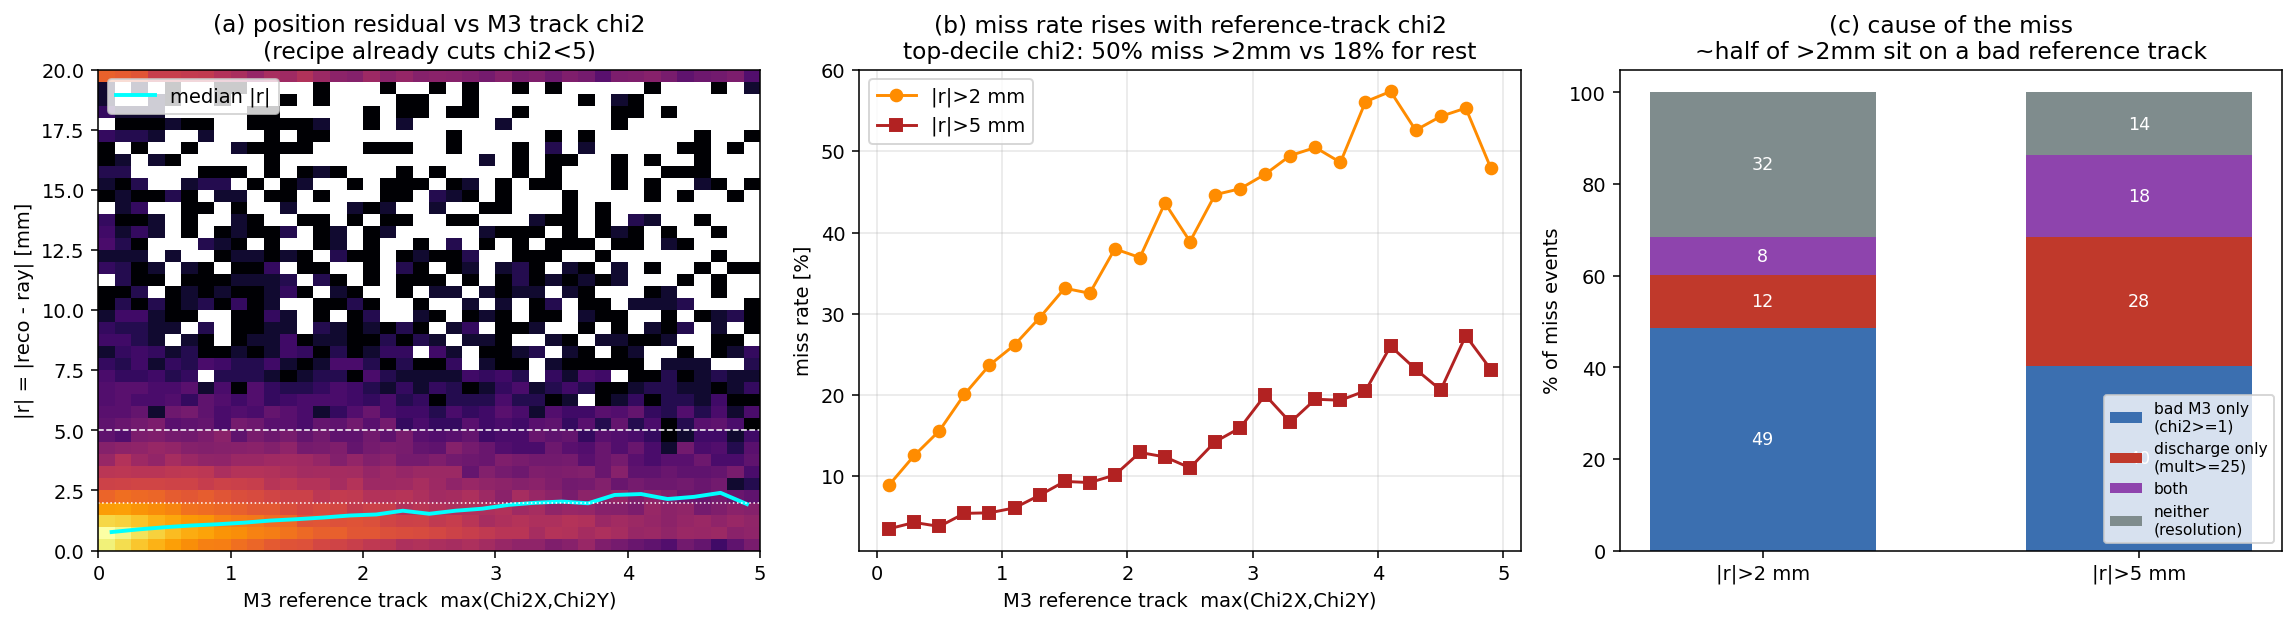
\includegraphics[width=\textwidth]{fig1_reference_fault_g_det3_wknd.png}
\caption{\textbf{Is it the reference tracker's fault?} (a) $|r|$ vs M3 track
$\max(\chi^2_X,\chi^2_Y)$; the median (cyan) climbs with reference-track $\chi^2$. (b) miss
rate vs M3 $\chi^2$ --- top-decile tracks miss $2.7\times$ more often. (c) cause attribution:
$\sim$half of the $>\!2$~mm misses occur on an elevated-$\chi^2$ reference track.}
\label{fig:ref}
\end{figure}

\section{Intrinsic chamber accuracy}
Removing the two pathologies isolates the chamber's true position accuracy
(Fig.~\ref{fig:intr}). Of \emph{all} reconstructed hits $93.2\%$ are within $5$~mm; requiring a
clean reference track ($\chi^2_{\max}<1$, $68\%$ of events) raises this to $\mathbf{95.8\%}$,
and additionally requiring no sub-spark discharge (mult $<25$, together $63\%$ of events) raises
it to $\mathbf{98.5\%}$. The chamber-side residual is the familiar mechanism: the $>\!5$~mm miss
rate is flat ($\sim3\%$) up to $\sim25$ strips and then climbs steeply toward the $50$-strip
spark veto (Fig.~\ref{fig:intr}c), i.e.\ sub-veto discharges throwing a displaced competing
cluster. Both effects reproduce on the independent \texttt{sat\_det3} run (490\,V/1000\,V):
within-$5$~mm $=93.6/95.9/98.4\%$ for all/clean-M3/clean-both, and top-decile M3-$\chi^2$
misses $48\%$ vs $18\%$.

\begin{figure}[h]\centering
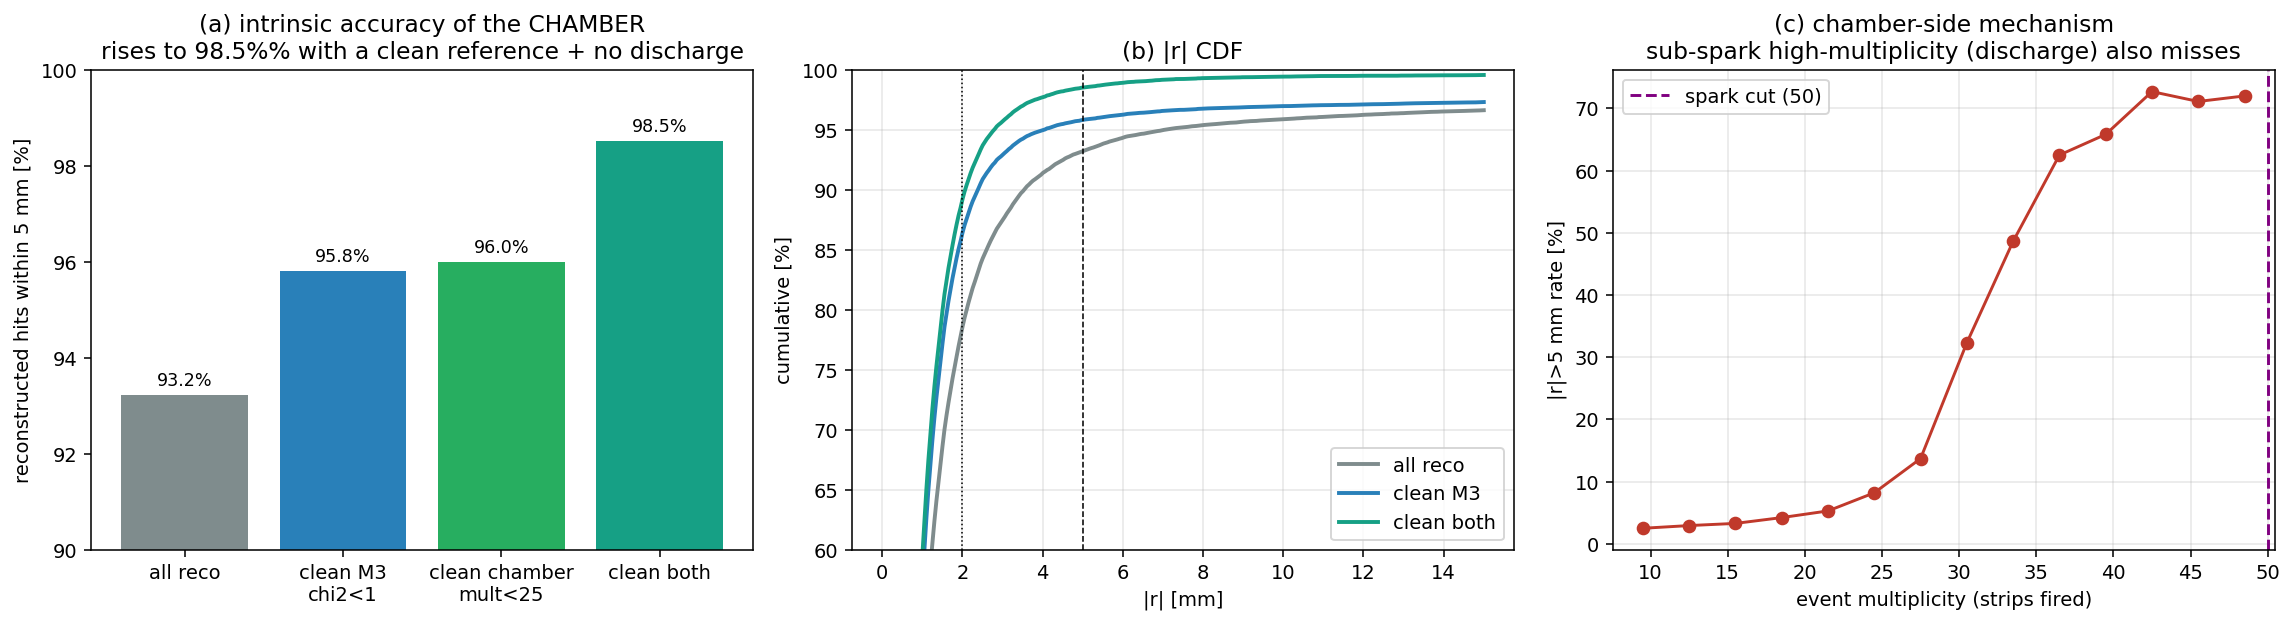
\includegraphics[width=\textwidth]{fig2_intrinsic_accuracy_g_det3_wknd.png}
\caption{\textbf{Intrinsic chamber accuracy.} (a) within-$5$~mm fraction rises $93.2\to98.5\%$
once reference and discharge pathologies are removed; (b) $|r|$ CDF for the same subsets;
(c) chamber-side mechanism --- miss rate climbs with multiplicity toward the spark veto.}
\label{fig:intr}
\end{figure}

\section{Q2 --- No edge enhancement in v2}
Mapping the miss rate against distance to the nearest active edge (Fig.~\ref{fig:edge}d), both
the $>\!2$~mm and $>\!5$~mm rates are \textbf{flat} across the chamber ($6.9\%$ within $10$~mm of
an edge vs $7.0\%$ in the bulk for $>\!5$~mm). The low-$X$/left-edge concentration reported in
the pre-v2 note was a property of the $\chi^2<20$ discharge tail; the v2 recipe removes it. The
only genuine edge effect is geometric acceptance and the passivated band (Q3), not a
mis-reconstruction hot-spot. This transfers to \texttt{sat\_det3} (edge-distance rates
$5.1$--$6.5\%$).

\section{Q3 --- The passivated $\sim2$~cm $Y$ strip is real, and already excluded}
Projecting every reference ray into the detector-local strip frame and profiling the efficiency
(Fig.~\ref{fig:edge}a--c) measures the active area directly:
%
\begin{itemize}\setlength\itemsep{0.1em}
  \item \textbf{Detector-local $Y$}: efficiency is dead below $Y\approx18$~mm and above
        $Y\approx380$~mm, flat ($\sim93\%$ plateau, spark excluded) in between. This is the
        \textbf{passivated band: $18.0$~mm at the low edge and $18.7$~mm at the high edge}
        ($\sim1.8$~cm each, matching the ``$\sim2$~cm'' recollection). Active $Y$ span
        $= 362$~mm of the nominal $399$~mm.
  \item \textbf{Detector-local $X$}: sharp geometric turn-on/off right at $0$ and $399$~mm,
        \emph{no} passivation. Active $X$ span $= 404$~mm (i.e.\ full width to alignment
        precision).
\end{itemize}
%
The passivation edges come out \emph{identical} on the independently-aligned \texttt{sat\_det3}
run ($18.0$/$18.6$~mm, active $Y=[18,380]$), confirming a real physical property of the
chamber rather than an alignment artefact.

\paragraph{Effect on the efficiency.} The good news: the current active box in
\texttt{09\_efficiency\_breakdown.py} is the $0.5$--$99.5$ percentile of \emph{reconstructed}
positions, and since reco only happens in the active $Y$ region, the box self-clips to
$\sim362$~mm in $Y$ and the passivated dead strips \textbf{never enter the denominator}.
Recomputing over the explicitly-measured active rectangle
($X\in[-3,400]$, $Y\in[18,380]$ mm) gives $88.4\%$ \reconear\ / $6.5\%$ \recofar\ / $4.6\%$
spark --- i.e.\ the headline $88.8\%$ is a genuine \emph{active-area} efficiency, not diluted
by passivation. For contrast, if one na\"ively used the nominal $40\times40$~cm the same
numerator over the full $399$~mm $Y$ would read only $\sim80\%$; the $\sim9\%$ passivated
$Y$ fraction must not be counted as inefficiency. Recommendation: keep reporting the
active-area efficiency, and \emph{document the measured active area}
($362\times404$~mm $\approx 36.2\times40.4$~cm, passivated $Y$ band $\approx18$~mm/side) so the
denominator is explicit rather than implicit in a percentile.

\begin{figure}[h]\centering
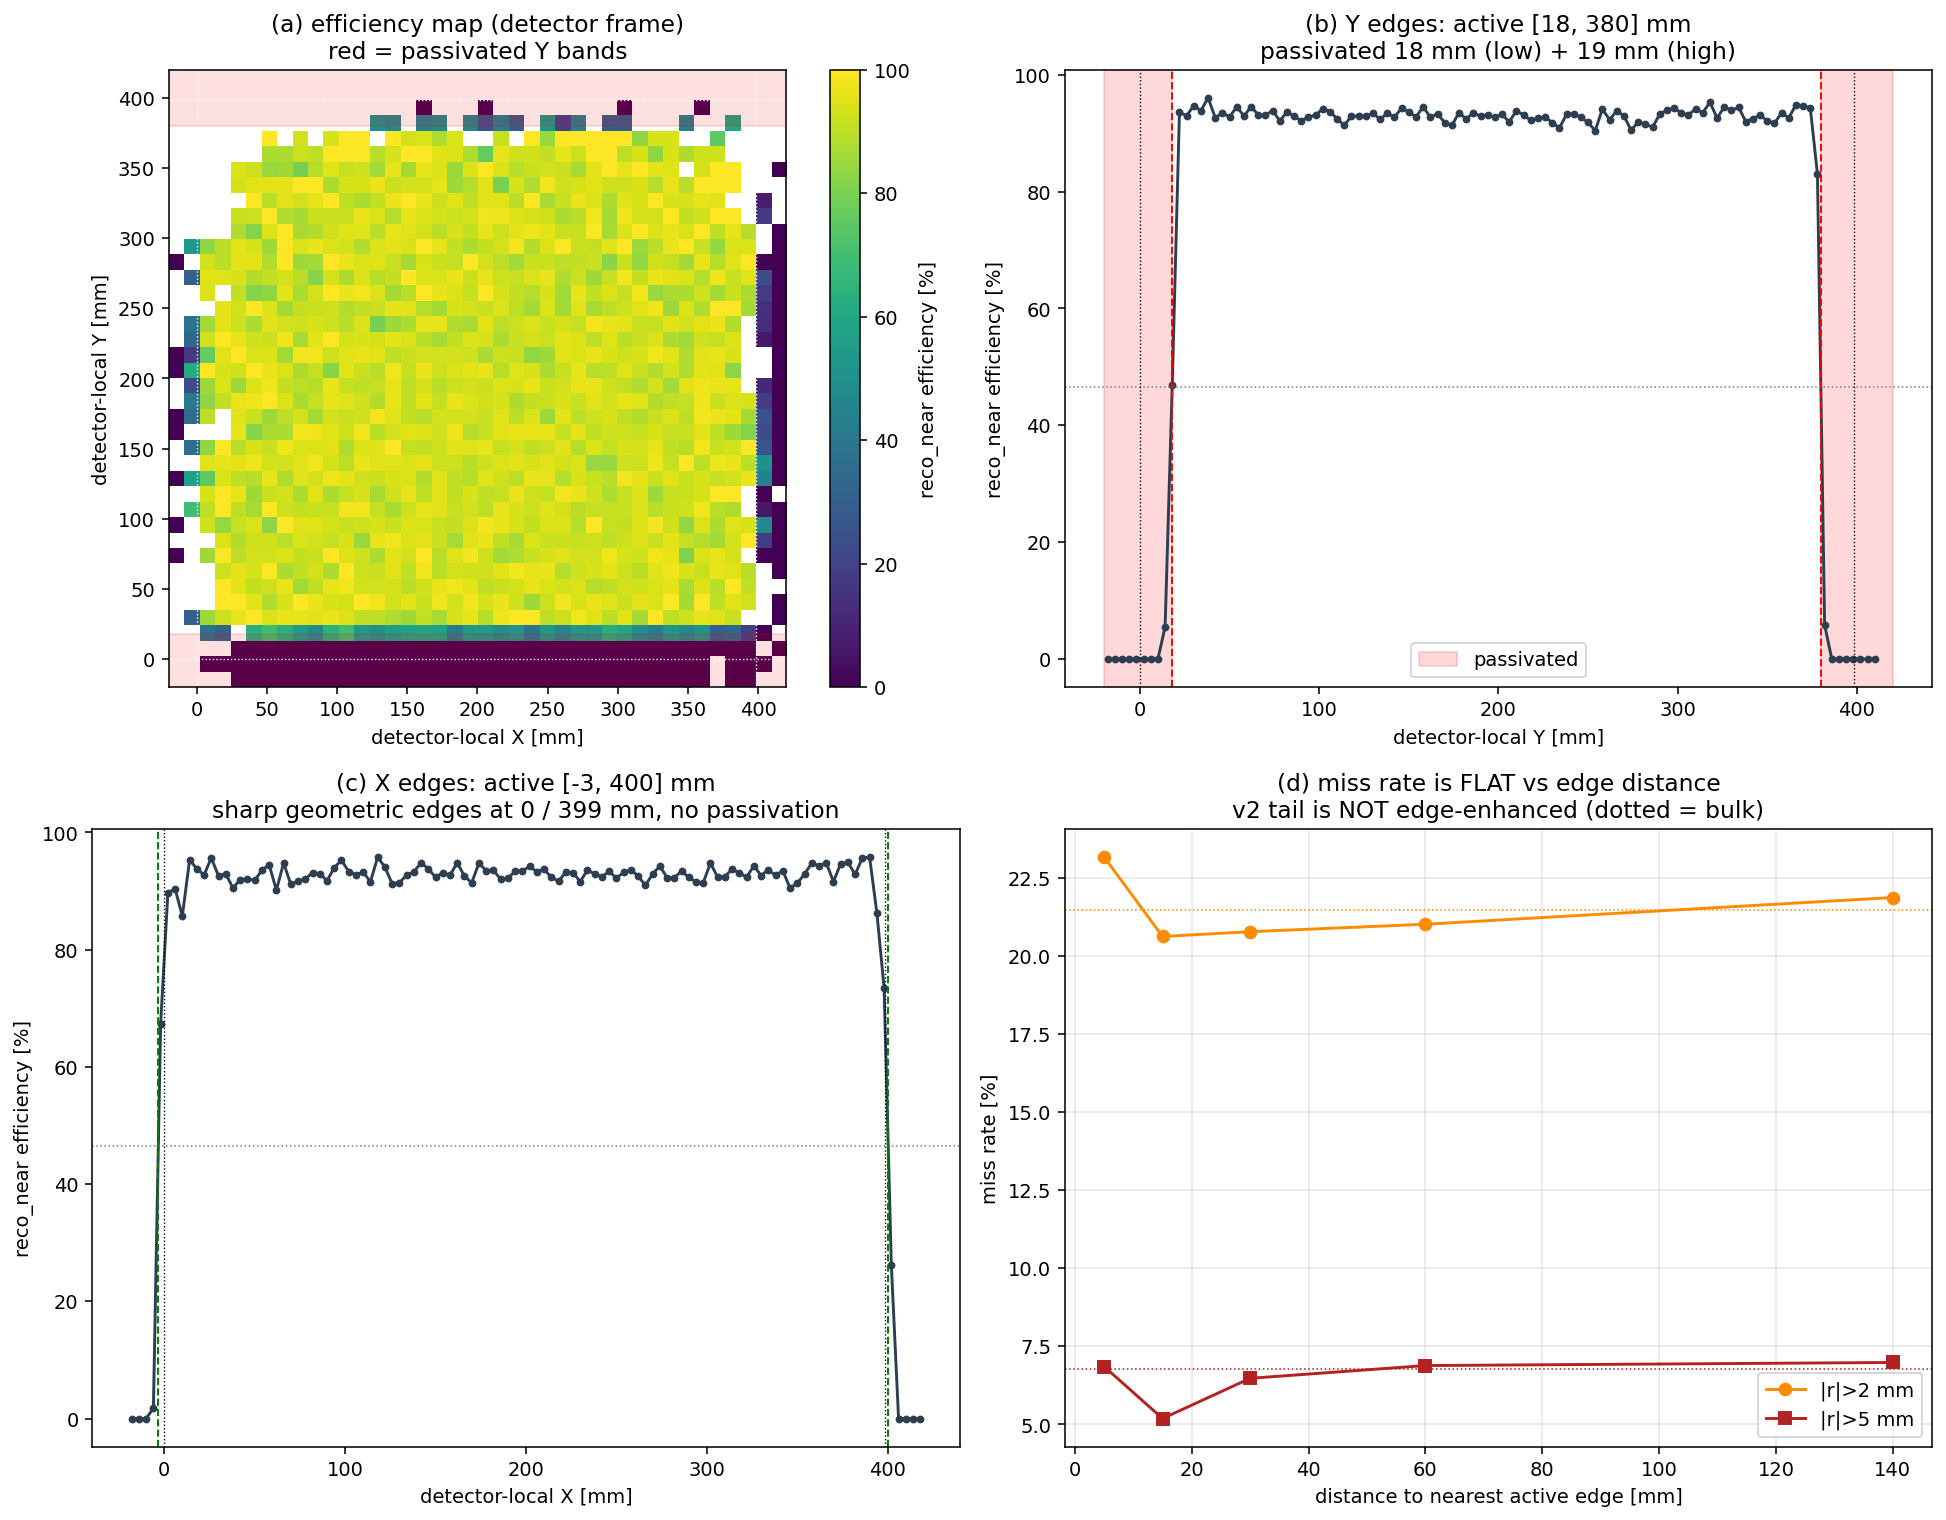
\includegraphics[width=0.95\textwidth]{fig3_edges_passivation_g_det3_wknd.png}
\caption{\textbf{Edges and passivation (detector-local frame).} (a) efficiency map; the red
bands are the passivated $Y$ strips (dead). (b) efficiency vs $Y$: active $[18,380]$~mm,
$\sim18$~mm passivated each side. (c) efficiency vs $X$: sharp geometric edges at $0/399$~mm,
no passivation. (d) miss rate vs distance to nearest active edge --- flat, i.e.\ the v2 tail is
not edge-driven (dotted $=$ bulk).}
\label{fig:edge}
\end{figure}

\section{Choosing a stricter reference cut for reprocessing}
Because the miss is reference-limited, the natural question is how strict an M3 cut we
should adopt. Our sample is already $\chi^2<5$, so we scan \emph{stricter}
(Fig.~\ref{fig:scan}), applying $\max(\chi^2_X,\chi^2_Y)\le T$ on both planes and tracking
the detector's core $\sigma(|r|<15)$, the \recofar\ rate, and the surviving statistics.

The detector core $\sigma$ falls monotonically from $0.626$~mm ($\chi^2<5$) to $0.457$~mm
($\chi^2<0.3$) with \textbf{no plateau} --- i.e.\ reference-tracker error still dominates the
measured residual across the whole $\chi^2<5$ band, so we ``can still see the difference'' even
at the tightest cut statistics allow. A differential fit ($\sigma^2 = \sigma_\mathrm{det}^2 +
b\langle\chi^2\rangle$) puts the detector-intrinsic core resolution at
$\sigma_\mathrm{det}\lesssim0.3$--$0.45$~mm (the cleanest thin bin measures $0.45$~mm directly),
versus the $0.63$~mm we currently quote --- the quoted number is inflated by $\gtrsim40\%$ by
reference error. Both runs give identical curves.

\paragraph{Recommendation.} Adopt \boxed{\chi^2<1.0 \text{ on both planes } +\ \mathrm{NClus}=4}
as the standard reprocessing cut. It captures the steep part of the improvement (core
$\sigma\,0.63\to0.47$~mm, $-25\%$; \recofar\ $6.8\to3.3\%$; within-$2$~mm $78.5\to89.5\%$) while
retaining $\sim43\%$ of tracks --- ample for the high-statistics June runs (tens of thousands of
crossings). If per-bin statistics are tight (fine 2-D maps) fall back to $\chi^2<1.0$,
NClus$\ge3$ ($68\%$ retained, $\sigma\,0.52$~mm). For the dedicated \emph{spatial-resolution}
number specifically, push tighter still ($\chi^2<0.5$, $\sigma\,0.48$~mm) or quote the
deconvolved intrinsic, since $\sigma$ has not converged. \textbf{Every June analysis
(efficiency, spatial resolution, angle) should be re-run on this cut} --- see
\texttt{M3\_CUT\_AND\_ACTIVE\_AREA\_NOTE.md}.

\begin{figure}[h]\centering
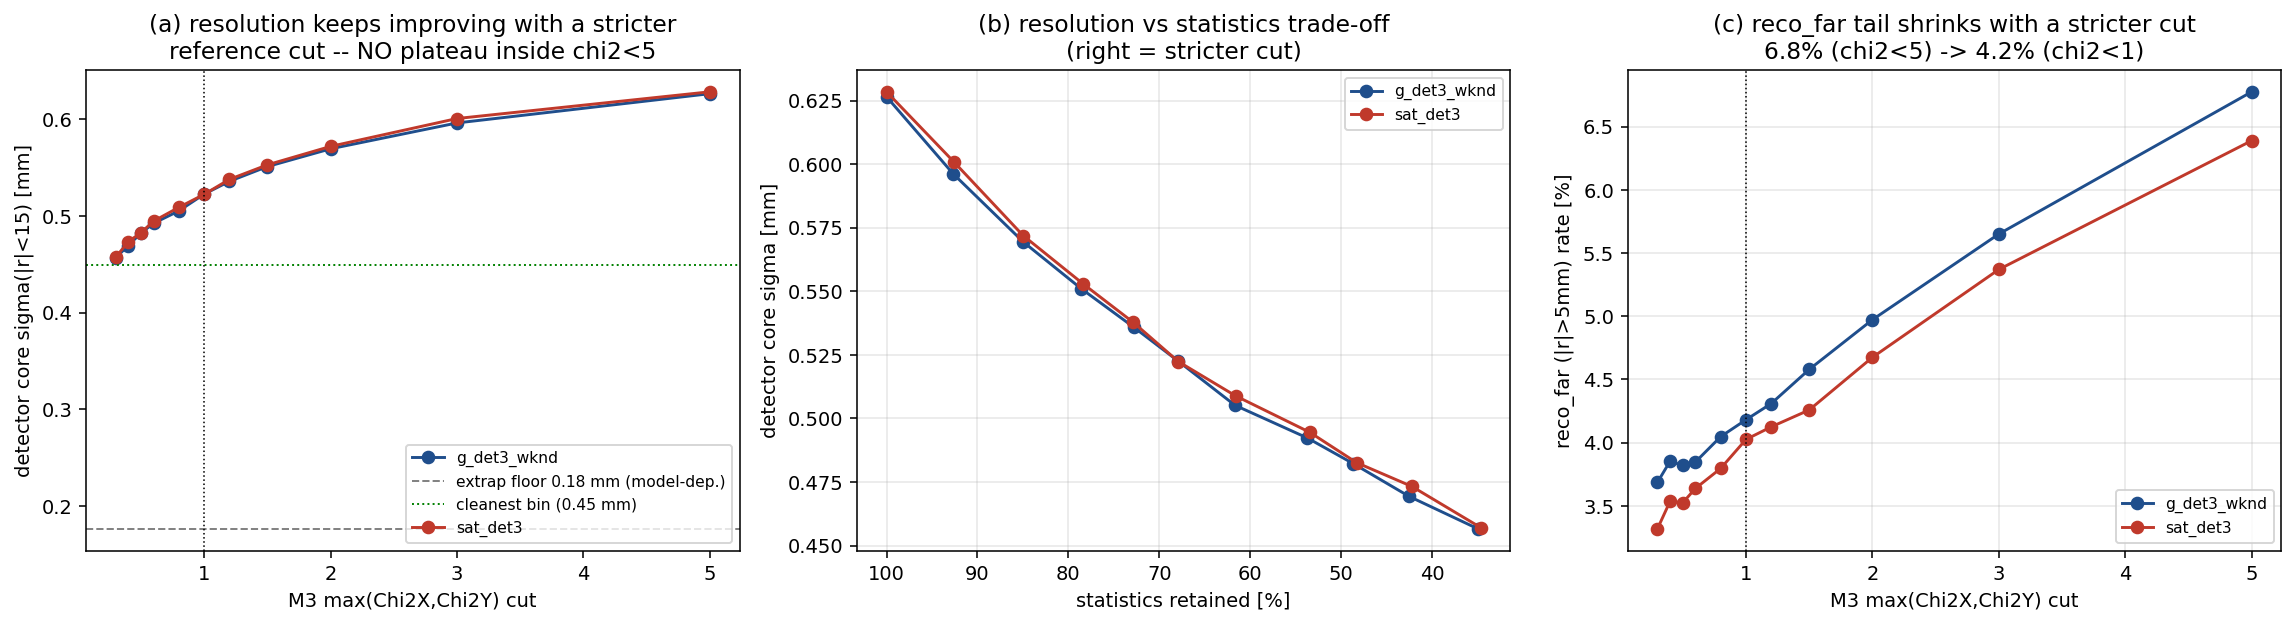
\includegraphics[width=\textwidth]{fig4_m3_cut_scan.png}
\caption{\textbf{Stricter reference cut.} (a) detector core $\sigma$ vs the M3 $\chi^2$ cut ---
no plateau; the quoted $0.63$~mm is reference-limited. (b) $\sigma$ vs statistics retained (the
trade-off; right $=$ stricter). (c) \recofar\ rate shrinks $6.8\to4.2\%$ from $\chi^2<5$ to
$\chi^2<1$.}
\label{fig:scan}
\end{figure}

\section{Takeaways}
\begin{itemize}\setlength\itemsep{0.15em}
  \item The $6.5\%$ \recofar\ (and the broader $21\%$ $>\!2$~mm) is \textbf{$\sim$half
        reference-tracker error} (elevated-$\chi^2$ M3 tracks that still pass the cut) and
        $\sim$half chamber-side sub-veto discharge, with a $\sim30\%$ ordinary-resolution
        shoulder just past the cut. It is \textbf{not} edge-localised and \textbf{not} a
        ray-matching or single-plane fault.
  \item The chamber's \emph{intrinsic} within-$5$~mm accuracy is $\mathbf{98.5\%}$
        (clean reference $+$ no discharge); the reported $93.2\%$ / core $\sigma=0.63$~mm are
        inflated by reference-tracker error ($\gtrsim40\%$ on $\sigma$). The measured residual is
        reference-limited with no plateau inside $\chi^2<5$ --- \textbf{reprocess everything on
        $\chi^2<1.0$ + NClus$=4$} (core $\sigma\to0.47$~mm at $43\%$ statistics); go tighter still
        for the dedicated resolution quote.
  \item The $\sim2$~cm passivated $Y$ band is confirmed and measured ($18$~mm/side); it is
        already excluded from the efficiency denominator, so $88.8\%$ is a true active-area
        number. Document the measured active area ($\approx36.2\times40.4$~cm) explicitly.
\end{itemize}

\vspace{0.4em}
\footnotesize\noindent\textit{Reproduce:} \texttt{edge\_chi2\_extract.py [KEY]} (v2 recipe;
records M3 track quality $+$ all-crossing categories over a wide window) then
\texttt{edge\_chi2\_plots.py [KEY]}; numbers in \texttt{edge\_chi2\_meta\_<KEY>.json}. Runs:
\texttt{g\_det3\_wknd} (headline) and \texttt{sat\_det3} (490\,V/1000\,V cross-check).
Categorisation matches \texttt{09\_efficiency\_breakdown.py}.

\end{document}
